

\documentclass{beamer}
 
\usepackage[utf8]{inputenc}
 \usetheme{Madrid}
 \usecolortheme{beaver}
 \usefonttheme{structuresmallcapsserif}
 \usepackage{listings}
%Information to be included in the title page:


\title[Distributed Systems] %optional
{Communication}

\subtitle{An Overview}

\author[Dr. Joseph Kehoe] % (optional, for multiple authors)
{Joseph Kehoe\inst{1}}

\institute[IT Carlow] % (optional)
{
	\inst{1}%
	Department of Computing and Networking\\
	Institute of Technology Carlow
}

\date[ITC 2018] % (optional)
{CDD101, 2018}

\logo{
\includegraphics[height=1.5cm]{../../itcarlowlogo.png}}




 
 \AtBeginSection[]
 {
 	\begin{frame}
 		\frametitle{Table of Contents}
 		\tableofcontents[currentsection]
 	\end{frame}
 }
 
 
 
\begin{document}
 
\frame{\titlepage}
 
  \begin{frame}
  	\frametitle{Table of Contents}
  	\tableofcontents
  \end{frame}
 

\section{Overview}
  \begin{frame}
  	\frametitle{Communication Overview}
  	Computers in a distributed system may have different:
  	\begin{itemize}
  		\item Architectures
  		\item Operating Systems
  		\item Data encoding
  		\item programming languages
  	\end{itemize}
We need a system of communication that allows them to talk to each other transparantly
  	
  		%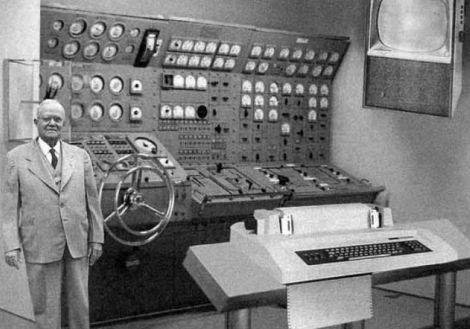
\includegraphics[height=4cm]{Old-Server.jpg}
  \end{frame}
  
\section{Protocols}

  \begin{frame}
  	\frametitle{Networking Protocols}
  	Communication between computers is build on existing network protocols
  	\begin{itemize}
  		\item At the base we have TCP/IP or UDP/IP
  		\item We can use socket programming to use these directly
  		\item Or we can use higher level protocols instead of or alongside this: e.g. HTTP
  		\item This base level protocol is available to all computers
  		\item But we will need to add a layer on top of this base in order to give us the extra features we need
  	\end{itemize}
I am going to assume you are familiar with these lower level protocols
  	
  	%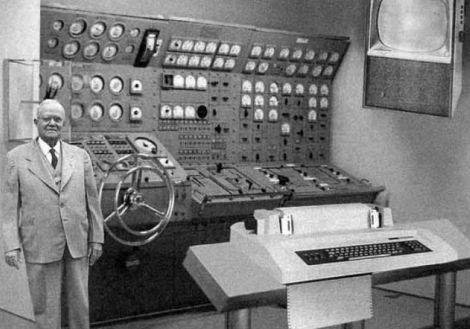
\includegraphics[height=4cm]{Old-Server.jpg}
  \end{frame}

\section{Remote Procedure Call}
  \begin{frame}
  	\frametitle{RPC}
  	Allow code to call procedures not resident on the local machine
  	\begin{itemize}
  		\item 
  	\end{itemize}
  	
  	
  	%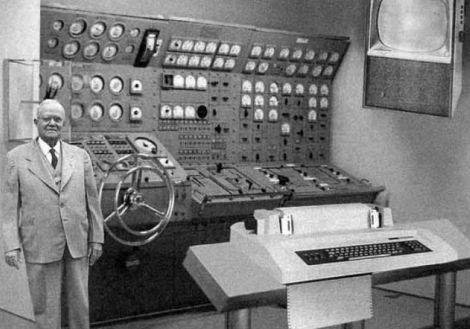
\includegraphics[height=4cm]{Old-Server.jpg}
  \end{frame}
  
\section{Remote Object Invocation}
\section{Messaging}

\end{document}

